% =============================================================================
% COPYRIGHT AND DISCLAIMER
% =============================================================================
% This file is provided as a convenience template for competition participants.
% By using it, you accept full responsibility for compliance with all applicable
% copyright, licensing, and usage rules of the Association for Computing
% Machinery (ACM) and of any LaTeX packages you load (including, without
% limitation, the "acmart" document class and related ACM materials).
%
% Consult ACM's official publication, template, and copyright policies before
% using this setup for any purpose other than this competition. Do not assume
% that this template may be reused, redistributed, or submitted elsewhere
% without independently verifying ACM's current rules.
%
% Use of the "acmart" class, the "sigconf" option, or ACM-style formatting in
% this template does NOT mean that this report, this competition, its organizers,
% or any resulting PDF is sponsored, endorsed, affiliated with, or published by
% ACM. ACM trademarks and branding remain the property of ACM.
%
% Template packages live in preamble.tex.
% Citations live in main.bib. Edit this file with your paper content.
% =============================================================================

\documentclass[sigconf]{acmart}
% =============================================================================
% Template setup — participants normally do not edit this file.
% Author content belongs in main.tex; citations belong in main.bib.
% \documentclass lives in main.tex so Overleaf does not treat this file as root.
% =============================================================================

% --- Competition / non-ACM-submission friendly rights metadata -------------
\setcopyright{none}
\settopmatter{printacmref=false}
\acmConference[Kaggle Competition]{Filament Segmentation Challenge}{2026}{\href{https://www.kaggle.com/competitions/filament-segmentation-2026}{kaggle.com/competitions/filament-segmentation-2026}}
\acmBooktitle{Competition Report}
\acmDOI{}
\acmISBN{}

% --- Author guidance text --------------------------------------------------
% \guide{...} is gray italic while \guideStyletrue; omitted from the PDF if false.
% Flip the switch in main.tex after % =============================================================================
% Template setup — participants normally do not edit this file.
% Author content belongs in main.tex; citations belong in main.bib.
% \documentclass lives in main.tex so Overleaf does not treat this file as root.
% =============================================================================

% --- Competition / non-ACM-submission friendly rights metadata -------------
\setcopyright{none}
\settopmatter{printacmref=false}
\acmConference[Kaggle Competition]{Filament Segmentation Challenge}{2026}{\href{https://www.kaggle.com/competitions/filament-segmentation-2026}{kaggle.com/competitions/filament-segmentation-2026}}
\acmBooktitle{Competition Report}
\acmDOI{}
\acmISBN{}

% --- Author guidance text --------------------------------------------------
% \guide{...} is gray italic while \guideStyletrue; omitted from the PDF if false.
% Flip the switch in main.tex after % =============================================================================
% Template setup — participants normally do not edit this file.
% Author content belongs in main.tex; citations belong in main.bib.
% \documentclass lives in main.tex so Overleaf does not treat this file as root.
% =============================================================================

% --- Competition / non-ACM-submission friendly rights metadata -------------
\setcopyright{none}
\settopmatter{printacmref=false}
\acmConference[Kaggle Competition]{Filament Segmentation Challenge}{2026}{\href{https://www.kaggle.com/competitions/filament-segmentation-2026}{kaggle.com/competitions/filament-segmentation-2026}}
\acmBooktitle{Competition Report}
\acmDOI{}
\acmISBN{}

% --- Author guidance text --------------------------------------------------
% \guide{...} is gray italic while \guideStyletrue; omitted from the PDF if false.
% Flip the switch in main.tex after \input{preamble}.
%
% Do not use \guide{...} for \email{...}.
\usepackage{xcolor}
\newif\ifguideStyle
\guideStyletrue
\newcommand{\guide}[1]{%
  \ifguideStyle
    {\color{gray!65}\itshape #1}%
  \fi
}

% --- Math ------------------------------------------------------------------
% Do NOT load amssymb (or amsfonts): acmart already loads newtxmath, which
% defines the same symbols (e.g. \Bbbk) and causes a conflict on Overleaf.
% amsmath is already provided by acmart; mathtools extends it.
\usepackage{mathtools}

% --- Figures ---------------------------------------------------------------
% graphicx is already loaded by acmart
\usepackage{subcaption}

% --- Tables ----------------------------------------------------------------
% booktabs is already loaded by acmart
\usepackage{tabularx}
\usepackage{multirow}

% --- Bibliography style is set in main.tex (ACM-Reference-Format) ----------
.
%
% Do not use \guide{...} for \email{...}.
\usepackage{xcolor}
\newif\ifguideStyle
\guideStyletrue
\newcommand{\guide}[1]{%
  \ifguideStyle
    {\color{gray!65}\itshape #1}%
  \fi
}

% --- Math ------------------------------------------------------------------
% Do NOT load amssymb (or amsfonts): acmart already loads newtxmath, which
% defines the same symbols (e.g. \Bbbk) and causes a conflict on Overleaf.
% amsmath is already provided by acmart; mathtools extends it.
\usepackage{mathtools}

% --- Figures ---------------------------------------------------------------
% graphicx is already loaded by acmart
\usepackage{subcaption}

% --- Tables ----------------------------------------------------------------
% booktabs is already loaded by acmart
\usepackage{tabularx}
\usepackage{multirow}

% --- Bibliography style is set in main.tex (ACM-Reference-Format) ----------
.
%
% Do not use \guide{...} for \email{...}.
\usepackage{xcolor}
\newif\ifguideStyle
\guideStyletrue
\newcommand{\guide}[1]{%
  \ifguideStyle
    {\color{gray!65}\itshape #1}%
  \fi
}

% --- Math ------------------------------------------------------------------
% Do NOT load amssymb (or amsfonts): acmart already loads newtxmath, which
% defines the same symbols (e.g. \Bbbk) and causes a conflict on Overleaf.
% amsmath is already provided by acmart; mathtools extends it.
\usepackage{mathtools}

% --- Figures ---------------------------------------------------------------
% graphicx is already loaded by acmart
\usepackage{subcaption}

% --- Tables ----------------------------------------------------------------
% booktabs is already loaded by acmart
\usepackage{tabularx}
\usepackage{multirow}

% --- Bibliography style is set in main.tex (ACM-Reference-Format) ----------


% Guide styling: \guideStyletrue = show gray italic hints; \guideStylefalse = omit them
% \guideStyletrue
\guideStylefalse

\begin{document}

\title{Candidates, Simulated Annotators and Refinement: Learning to Select Filament Instances}  % Replace this with your title
\subtitle{A Solution to the Solar Filament Segmentation Challenge 2026} % DO NOT CHANGE


\author{Hibiki8739}
\affiliation{%
  \institution{Independent participant}
  \country{}
}
%

\begin{abstract}
    This report describes our solution to the Solar Filament Segmentation Challenge~2026, a Kaggle competition on automatic segmentation of solar filaments in GONG H-$\alpha$ observations. Instead of thresholding one probability map, we generate about 157 candidate regions per image from an ensemble of three dense networks, describe every candidate (map and shape statistics, agreement with an annotator-conditioned network that simulates the annotators, agreement with two Mask R-CNN detectors), and let a gradient-boosted model predict the expected matched IoU of each candidate, which is the quantity the panoptic-quality metric rewards. The selected instances are redrawn by three refiner networks in oriented crops and re-scored by a second model. In five-fold cross-validation on the 707 annotated training images the pooled panoptic quality is 0.462 (95\,\% interval [0.453, 0.471]); the public leaderboard score is 0.40. All code, the trained weights, and a notebook that reproduces the submission without retraining are public.
\end{abstract}

\maketitle

\ifguideStyle
\noindent{\color{gray!65}\itshape
Guide mode is on.}
\par\medskip
\fi

\guide{Please limit your report to four (4) pages, excluding the Acknowledgment and References sections. Throughout this document, please follow these considerations:
\begin{itemize}
    \item Do not alter any text that is currently in black color (except for the emails under authors' name).
    \item Replace all gray text with your own.
    \item When you are done with the report, please replace \texttt{\textbackslash guideStyletrue} with \texttt{\textbackslash guideStylefalse}, to remove any gray text. Alternatively, you can remove any text wrapped in \texttt{\textbackslash guide\{\}},
    \item Be as succinct as possible, and only provide details regarding your own work. For example, there is no need to discuss what solar filaments are, or why filament segmentation matters.
    \item If you must, you can add extra sections.
\end{itemize}}


% ==================================== %
%              INTRODUCTION            %
% ==================================== %
\section{Introduction}
    This report goes over the details of our submitted solution to the Solar Filament Segmentation Challenge~2026 \cite{filament-segmentation-2026}. The challenge, launched on July~10,~2026, is organized by the Earth-Space AI Research (ESAIR) Lab\footnote{\href{https://www.esairlab.com/home}{www.esairlab.com/}}. This challenge utilizes the MAGFiLO dataset for evaluation of the segmentation algorithms \cite{ahmadzadeh2024dataset}.
    Three properties of the task shaped our solution. (i)~The metric is panoptic quality (PQ) pooled over \emph{annotator records}: every record of an image is matched one-to-one against all predictions of the image (IoU\,$>$\,0.5). A prediction is therefore worth keeping only if its expected matched IoU, averaged over the records, exceeds PQ/2; this is a selection problem, not a thresholding problem. (ii)~The annotators differ in style (how many filaments, how wide the outline); 58\,\% of the training images have one record, the test images 2.4 on average. (iii)~Outline accuracy matters: dilating or eroding all our outlines by one pixel lowers the out-of-fold PQ by 0.02--0.03. Our pipeline (Fig.~\ref{fig:pipeline}) addresses (i) with a learned quality model over a large candidate pool, (ii) with simulated annotators, and (iii) with a stage-2 refiner.

\begin{figure}[t]
  \centering
  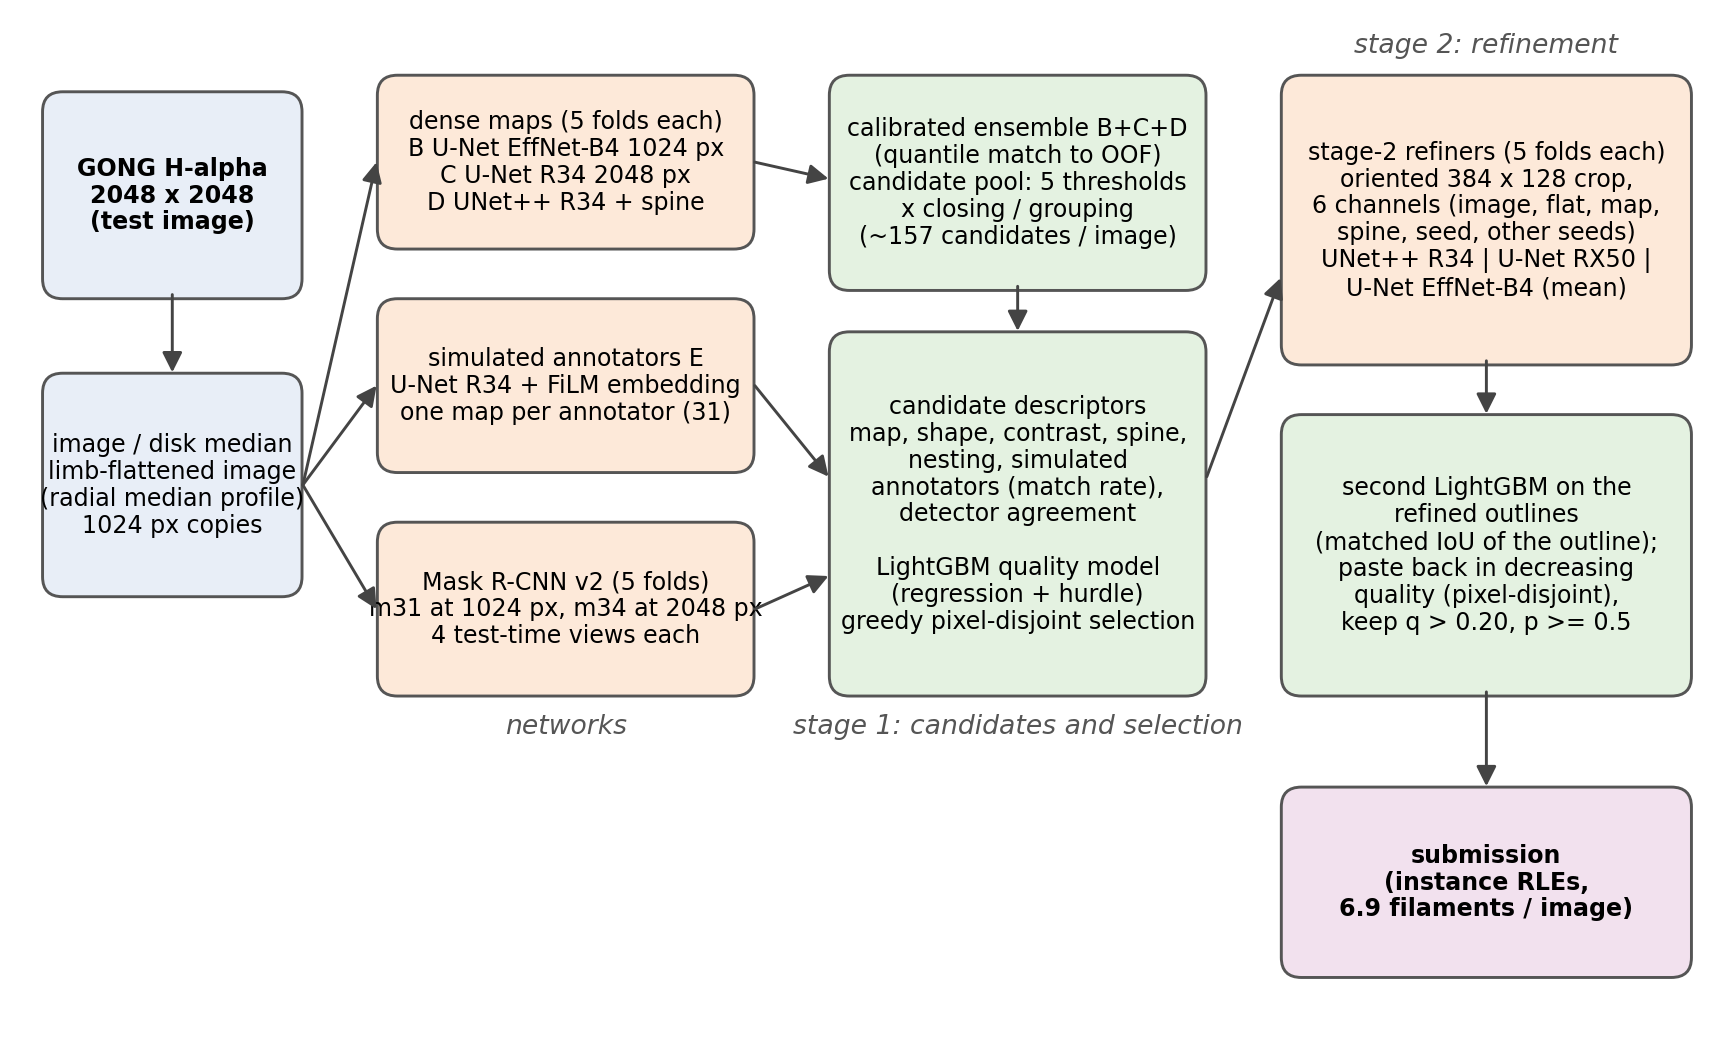
\includegraphics[width=\linewidth]{figures/pipeline.png}
  \caption{Data pipeline at test time. All networks are trained with the same five folds; at test time the five fold models are averaged.}
  \label{fig:pipeline}
\end{figure}

% ==================================== %
%              METHODOLOGY             %
% ==================================== %
\section{Methodology}\label{sec:methodology}

\textbf{Data and splits.} We use only the competition data: 707 training images (2048\,$\times$\,2048 px) with 1--3 annotator records each, 180 test images. All stages use the same five folds (a fixed random permutation of the sorted image names), so every training image has \emph{out-of-fold} (OOF) predictions from models that never saw it; all model selection uses the OOF PQ computed exactly like the competition metric (we verified our implementation against the organizers' self-evaluation notebook). No external annotations, no file-name metadata and no test-time information beyond the test images are used.

\textbf{Pre-processing.} Images are divided by their disk median brightness. A second channel removes limb darkening: the disk centre and radius are estimated from the image, the median brightness in 120 radial rings is interpolated to every pixel, and the image is divided by it (clipped to [0.4, 1.4]), so faint filaments near the limb get the contrast of disk-centre ones.

\textbf{Dense networks.} The target is the \emph{soft annotator mean} (fraction of an image's records that cover a pixel); images with several records are sampled twice as often, because the test set is dominated by them. B: U-Net with EfficientNet-B4 encoder at 1024 px; C: U-Net/ResNet34 with the flattened channel, trained on 1024 px crops of the native frames (70\,\% centred near a filament) and applied at 2048 px; D: UNet++/ResNet34 with a second output, the rasterised annotator \emph{spines}, BCE + 0.5 soft Dice + 0.3 spine BCE, EMA weights. Test-time augmentation uses flips (B) or all eight dihedral views (C, D). The test maps (mean of five fold models, smoother than an OOF map) are quantile-matched to the OOF value distribution, so thresholds and descriptors mean the same at test time.

\textbf{Simulated annotators.} Network E is a U-Net/ResNet34 whose encoder stages and decoder output are modulated by a learned embedding of the annotator (FiLM, identity-initialised); one training sample is one annotator record, 15\,\% of the samples use an ``unknown'' embedding. At test time E draws one map for each of the 31 annotators with at least eight records; for each candidate we count how many simulated annotators draw a component matching it (IoU\,$>$\,0.5) at three probability levels, separately for the annotators who worked in teams (the test set is team-annotated).

\textbf{Detectors.} Two Mask R-CNN v2 models (ResNet50-FPN, COCO initialisation, one record per sample): m31 at 1024 px and m34 trained on 1024 px crops and applied to the full 2048 px frame. Their instances (four test-time views $\times$ five folds) are not used as predictions but as evidence for the candidates (best IoU, score of the best match, coverage, number of overlapping instances, view disagreement).

\textbf{Candidate pool.} The calibrated mean map of B, C, D is thresholded at 0.2--0.6 (5 levels); for each level we take connected components as they are, after closing gaps with an 11 or 25 px disk, and groups of nearby pieces (41 or 61 px closing at quarter resolution). Components $\geq$150 px give about 157 overlapping candidates per image (110\,514 in the training set); the best possible selection from this pool reaches OOF PQ 0.55, our selection 0.46.

\textbf{First quality model.} Each candidate gets 75 descriptors: probability statistics, member disagreement, spine statistics, shape (area, solidity, elongation, width, fragments, holes), image contrast inside vs.\ around, nesting with other candidates, the simulated-annotator and detector descriptors. The target is the mean over the image's records of the matched IoU (0 if IoU\,$\leq$\,0.5). We average a LightGBM regression and a hurdle model ($P(\text{match}) \times E[\text{IoU}\mid\text{match}]$). Candidates are then taken greedily in decreasing predicted quality, skipping those that overlap an already taken one, down to quality 0.10 (a superset of all useful selections).

\textbf{Stage-2 refinement.} Each selected instance is cut out in an oriented 384\,$\times$\,128 crop (principal axis horizontal, at most 2$\times$ magnification) with six channels: image, flattened image, calibrated map, spine map, the instance (seed) and the other seeds. Three networks (UNet++/ResNet34, U-Net/ResNeXt50, U-Net/EfficientNet-B4; trained on the seeds of earlier selections, 8--10k steps, EMA) redraw the outline; their mean probability is thresholded at 0.40, only components touching the seed are kept, and an instance whose outline collapses below half of its seed is dropped. Outlines are pasted back in decreasing quality, so predictions never overlap (Fig.~\ref{fig:refine}).

\textbf{Second quality model.} The refined outline is described again (area change, IoU with the seed, mean and quantiles of the refined probability, soft margin, overlap with better instances) and a second LightGBM predicts its matched IoU. Out of fold, the second-stage prediction ranks the refined instances better than the first-stage quality or their mean, so it orders the instances; instances above 0.20 with mean refined probability $\geq$\,0.5 form the submission (6.5 per image out of fold, 6.9 per test image). All thresholds were chosen on OOF PQ.

\begin{figure*}[t]
  \centering
  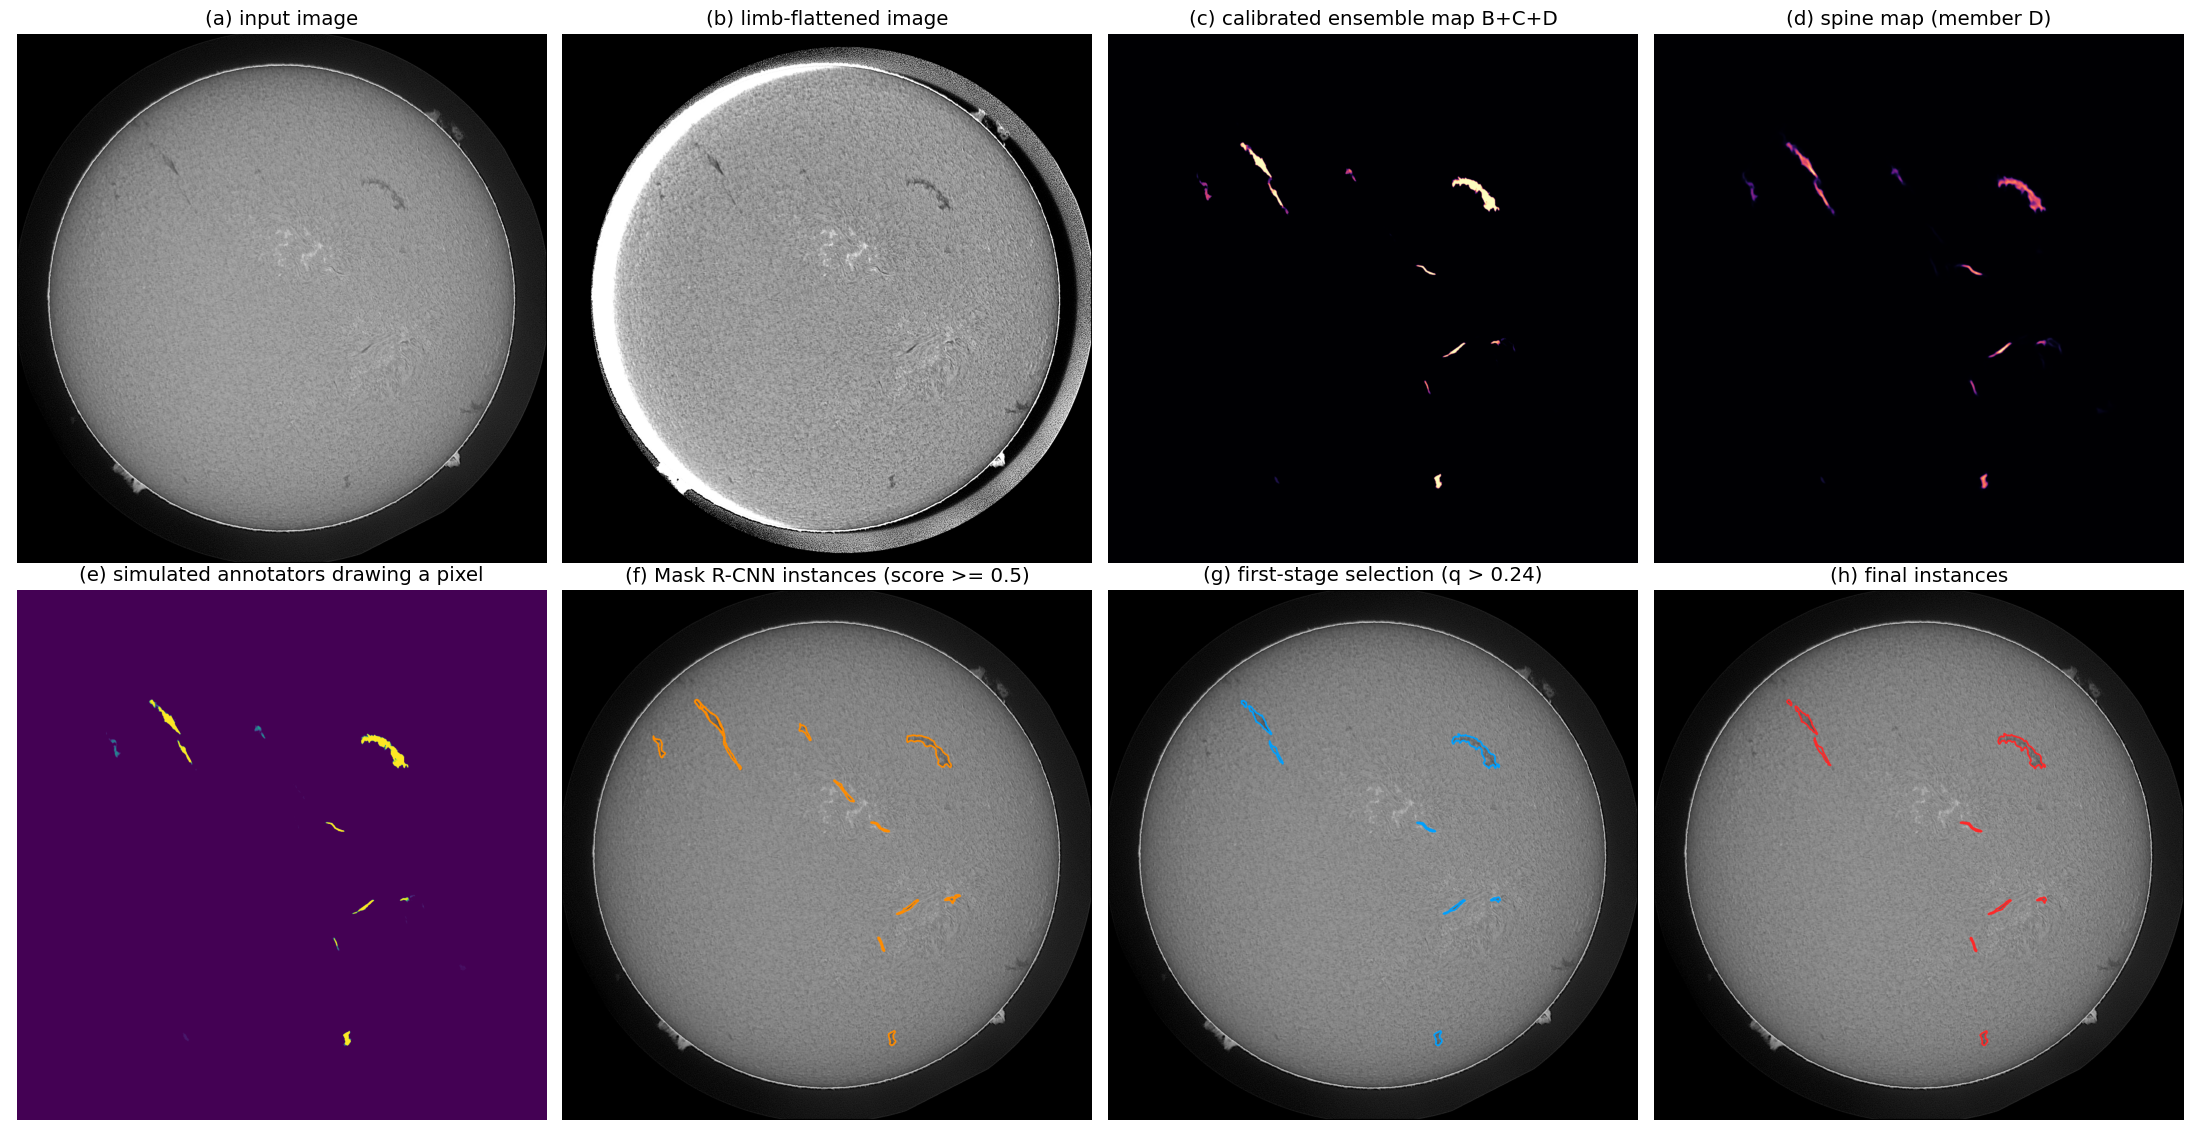
\includegraphics[width=\textwidth]{figures/stages.png}
  \caption{One test image through the pipeline. (c) calibrated B+C+D map, (d) spine map of D, (e) number of simulated annotators drawing a pixel, (f) Mask R-CNN instances, (g) first-stage selection, (h) final instances after refinement and re-scoring.}
  \label{fig:stages}
\end{figure*}

\begin{figure}[t]
  \centering
  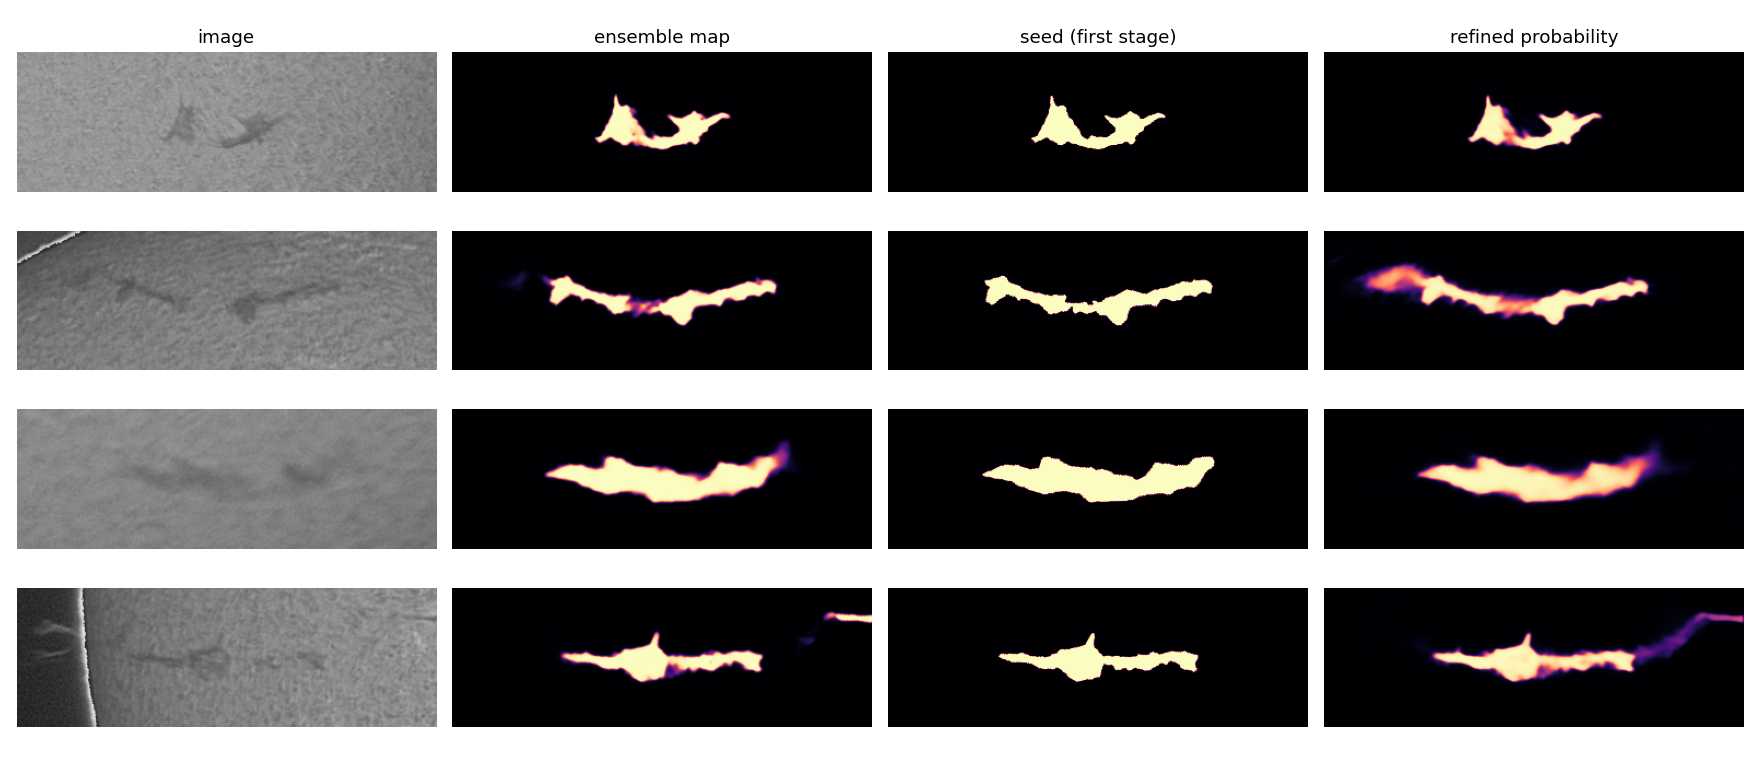
\includegraphics[width=\linewidth]{figures/refine.png}
  \caption{Stage-2 refinement on test instances: oriented crop of the image, calibrated ensemble map, first-stage instance (seed) and the mean probability of the three refiners.}
  \label{fig:refine}
\end{figure}

% ==================================== %
%              EVALUATION              %
% ==================================== %
\section{Evaluation}\label{sec:evaluation}
\textbf{Strategy.} Every number below is the pooled PQ over all annotator records of the OOF predictions of the 707 annotated training images (the competition metric), unless stated otherwise. Each stage is compared with its predecessor on the same folds and the same candidates; the 95\,\% interval is a bootstrap over images (2000 resamples). The public leaderboard was used as a sanity check only: its scores are shown with two decimals and were consistently 0.055--0.06 below OOF for every submission we made (including deliberate probes such as one-pixel dilation), i.e.\ the OOF ranking transferred.

\begin{table}[t]
  \caption{Out-of-fold PQ (all records pooled) as the pipeline grows. Each row adds one component to the row above.}
  \label{tab:ablation}
  \small
  \begin{tabular}{lr}
    \toprule
    Selection & OOF PQ \\
    \midrule
    member A, fixed rule (t\,=\,0.4, closing, $\geq$\,600 px) & 0.392 \\
    member A, learned quality model + greedy & 0.428 \\
    \midrule
    B+C+D pool, map / shape / contrast descriptors & 0.440 \\
    \quad + simulated annotators, regression+hurdle & 0.444 \\
    \quad + Mask R-CNN m31 evidence (4 views) & 0.455 \\
    \quad + Mask R-CNN m34 (2048 px), mean with m31 & 0.458 \\
    \quad + three stage-2 refiners & 0.460 \\
    \quad + second quality model (final) & \textbf{0.462} \\
    \bottomrule
  \end{tabular}
\end{table}

\begin{table}[t]
  \caption{Final pipeline, out of fold. K: annotator records per image. SQ: mean IoU of the matches; RQ: TP/(TP+FP/2+FN/2); 1:n / n:1: share of annotated filaments touched by several predictions / predictions touching several filaments (IoU $>$ 0).}
  \label{tab:final}
  \small
  \begin{tabular}{lrrrrrr}
    \toprule
     & PQ & SQ & RQ & Dice$_\text{match}$ & 1:n & n:1 \\
    \midrule
    all & 0.462 & 0.682 & 0.677 & 0.808 & 0.023 & 0.024 \\
    K = 1 & 0.466 & 0.687 & 0.678 & 0.811 & 0.022 & 0.027 \\
    K $\geq$ 2 & 0.459 & 0.679 & 0.677 & 0.805 & 0.024 & 0.022 \\
    \bottomrule
  \end{tabular}
\end{table}

\begin{figure}[t]
  \centering
  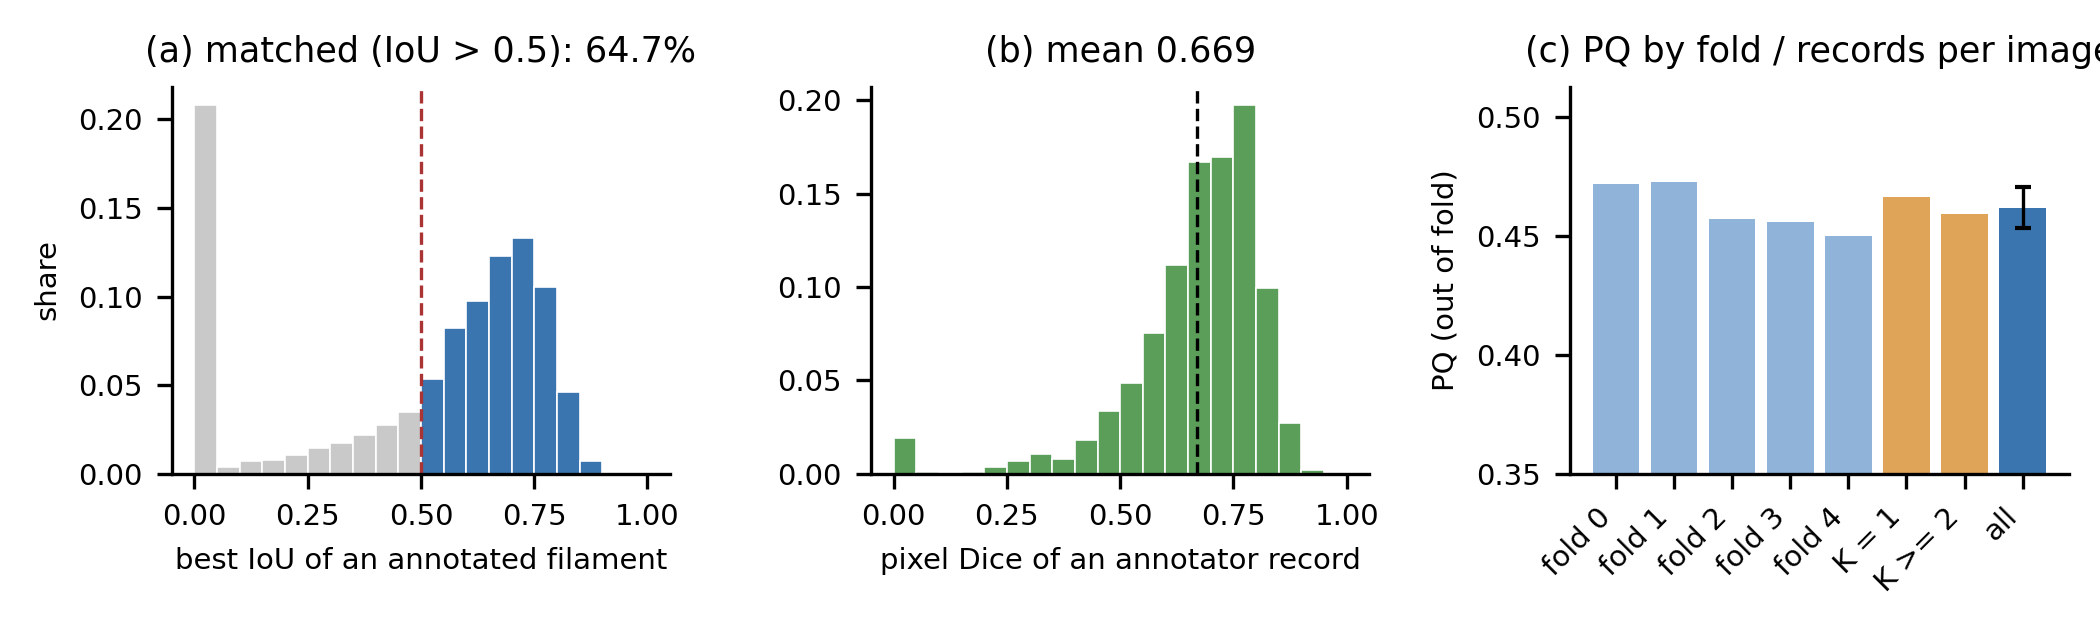
\includegraphics[width=\linewidth]{figures/eval.png}
  \caption{Out-of-fold evaluation of the final pipeline. (a) Best IoU of every annotated filament with any prediction (blue: matched). (b) Pixel Dice between the union of the predictions and the union of one record's filaments. (c) PQ per fold and per number of records; error bar: 95\,\% bootstrap interval over images.}
  \label{fig:eval}
\end{figure}

\begin{figure*}[t]
  \centering
  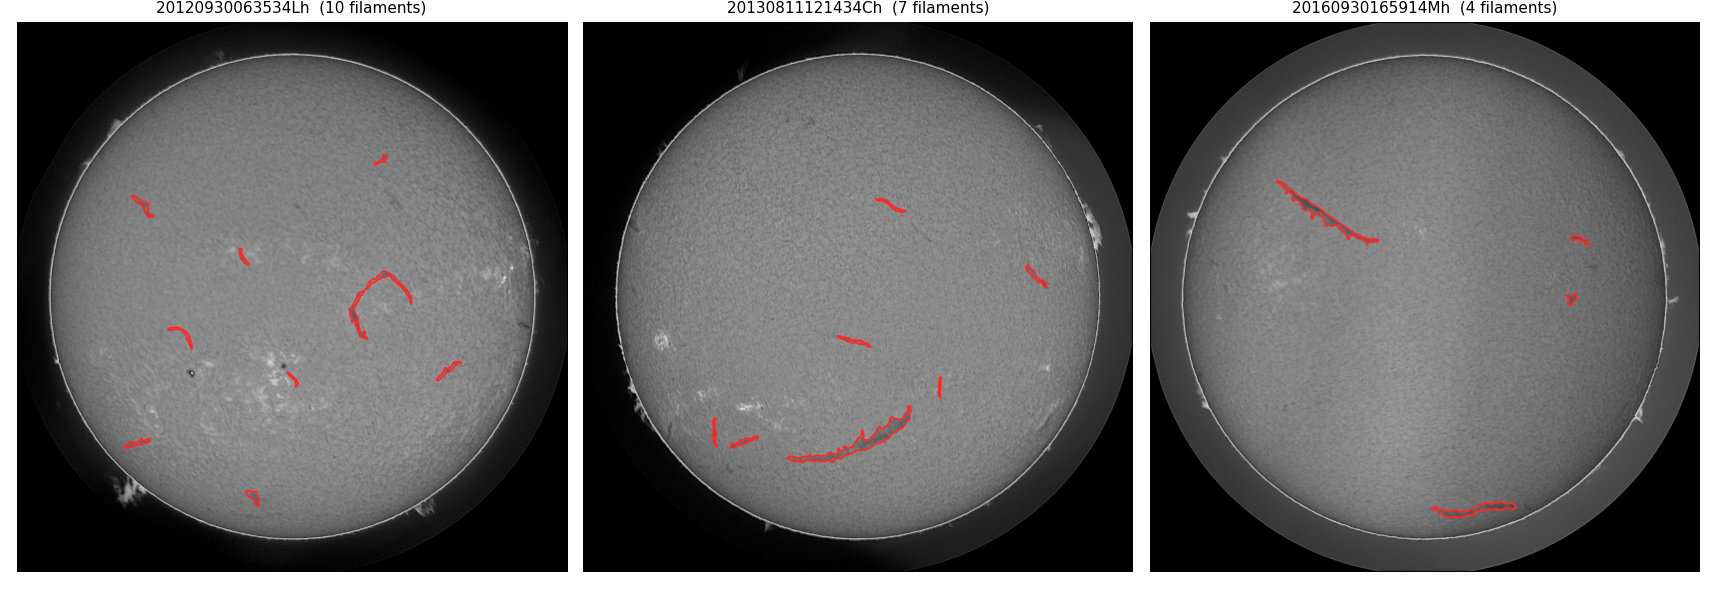
\includegraphics[width=\textwidth]{figures/examples.png}
  \caption{Final instances (red) on three test images with a low, median and high number of predicted filaments.}
  \label{fig:examples}
\end{figure*}

\textbf{What did not help} (OOF, same folds): 13 instead of 5 thresholds ($-$0.002 to $-$0.004: the oracle rises, the learned selection gets noisier), exact maximum-weight independent-set selection instead of greedy ($\pm$0.0005), weighting by the number of records ($-$0.0015), member E as a fourth dense member ($-$0.003), the detector instances as additional candidates ($-$0.0017), annotator identity as a feature (an oracle that knows the true annotator gains only 0.005), dilation/erosion of the outlines ($-$0.02 per pixel), and solar-physics descriptors (heliographic latitude\slash longitude and foreshortening, tilt mirrored by hemisphere, catalogue-style fragment-linkage geometry, sunspot cues; $-$0.0013). Bridging the fragments of multi-piece candidates lowers their quality (0.254$\to$0.221): annotators draw each filament as one connected polygon (8196 of 8198), and most misses are filaments that the annotator outlined much wider or fainter than our maps, not unlinked fragments.

\textbf{Strengths and weaknesses.} The quality model turns the metric's per-instance trade-off into a learned decision and absorbs new evidence cheaply (each detector or descriptor family is a few columns); the refiner improves outlines without fragmenting or merging instances (one-to-many and many-to-one rates stay at about 3\,\%). Weaknesses: 35\,\% of the annotated filaments are not matched and 21\,\% are not touched by any prediction (Fig.~\ref{fig:eval}a; mostly small, faint, or near the limb, where the candidate pool matches only 21\,\% of the filaments beyond 0.9\,$R_\odot$), the pipeline is heavy (9 networks $\times$ 5 folds, about 2.1\,h of inference on two T4 GPUs), and the annotator-style variance caps the attainable score (two human records agree at PQ 0.34). Improvements we would try next: candidates from the refiner itself (a second pool around low-quality regions), and limb-aware augmentation for the faint near-limb filaments.

{\sloppy \textbf{Reproducibility.} The repository (\href{https://github.com/hibiki-iwanaga/solar-filament-segmentation-2026}{github.com/\allowbreak hibiki-iwanaga/\allowbreak solar-\allowbreak filament-\allowbreak segmentation-2026}) contains the training notebooks of every stage, the weights (float16, 5 folds), the two LightGBM models and the calibration histograms; \texttt{pipeline.ipynb} produced the submitted file from the test images alone.\par}

% ==================================== %
%            ACKNOWLEDGMENT            %
% ==================================== %
\section{Acknowledgment}\label{sec:acknowledgment}
    % Do not change
    The organization of the Filament Segmentation Challenge 2026 is partially supported by the U.S. National Science Foundation (NSF) under Grant No. 2209912 and 2433781, directorate for Computer and Information Science and Engineering (CSE), and Office of Advanced Cyberinfrastructure (OAC), and Grant No. 2511630, AST Division Of Astronomical Sciences and MPS Directorate for Mathematical and Physical Sciences.

    The Filament Segmentation Challenge 2026 is sponsored by the U.S. National Science Foundation (NSF) National Solar Observatory (NSO).

    This work utilizes GONG data obtained by the NSO Integrated Synoptic Program, managed by the National Solar Observatory, which is operated by the Association of Universities for Research in Astronomy (AURA), Inc. under a cooperative agreement with the National Science Foundation and with contribution from the National Oceanic and Atmospheric Administration. The GONG network of instruments is hosted by the Big Bear Solar Observatory, High Altitude Observatory, Learmonth Solar Observatory, Udaipur Solar Observatory, Instituto de Astrofísica de Canarias, and Cerro Tololo Interamerican Observatory.

\bibliographystyle{ACM-Reference-Format}
\bibliography{main}

\end{document}
